\chapter{Hyperparameters}
\section{K-Means}
For selecting the appropriate amount of clusters, we used the silhouette method. 
Using this method, we ran the K-Means method multiple times for different $k$ values.
The results are plotted using a line-plot, and we select the highest silhouette score from this plot. 
\begin{enumerate}
  \item Seeds dataset (All dimensions): k-clusters.
  \begin{enumerate}
      \item 2-dimensions k-value: 2
      \item 3-dimensions k-value: 5
      \item 7-dimensions k-value: 2
  \end{enumerate}
      \item Heart dataset:
      \begin{enumerate}
          \item 2-dimensions k-value: 2
          \item 3-dimensions k-value: 4
          \item 9-dimensions k-value: 2
      \end{enumerate}
      \item Circle dataset:
      \begin{enumerate}
          \item 2-dimensions k-value: 7
          \item 3-dimensions k-value: 9
      \end{enumerate}
      \item Line dataset:
      \begin{enumerate}
          \item 2-dimensions k-value: 2
          \item 3-dimensions k-value: 2
      \end{enumerate}
      \item Skewed dataset:
      \begin{enumerate}
          \item 2-dimensions k-value: 5
          \item 3-dimensions k-value: 4
      \end{enumerate}
  \end{enumerate}

\newpage
\subsection{Seeds dataset}
\begin{figure}[H]
  \includegraphics[width=0.75\textwidth]{Method/images//k-values/seeds-dataset-2-kmeans.png}
  \caption{Selecting the $k$ for K-Means clustering for seeds dataset (2 dimensions) using the "silhouette method"}
  \label{hyperparameters:agglomerative-seeds-dataset-2d}
\end{figure}
\begin{figure}[H]
  \includegraphics[width=0.75\textwidth]{Method/images/k-values/seeds-dataset-2-kmeans.png}
  \caption{Selecting the $k$ for K-Means clustering for seeds dataset (3 dimensions) using the "silhouette method"}
  \label{hyperparameters:agglomerative-seeds-dataset-3d}
\end{figure}
\begin{figure}[H]
  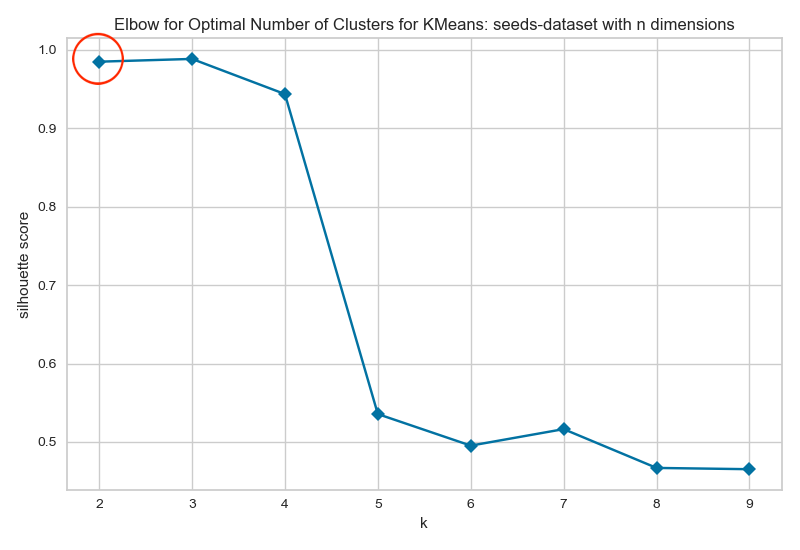
\includegraphics[width=0.75\textwidth]{Method/images/k-values/seeds-dataset-n-kmeans.png}
  \caption{Selecting the $k$ for K-Means clustering for seeds dataset (7 dimensions) using the "silhouette method"}
  \label{hyperparameters:agglomerative-seeds-dataset-7d}
\end{figure}
\newpage

\subsection{Heart dataset}
\begin{figure}[H]
  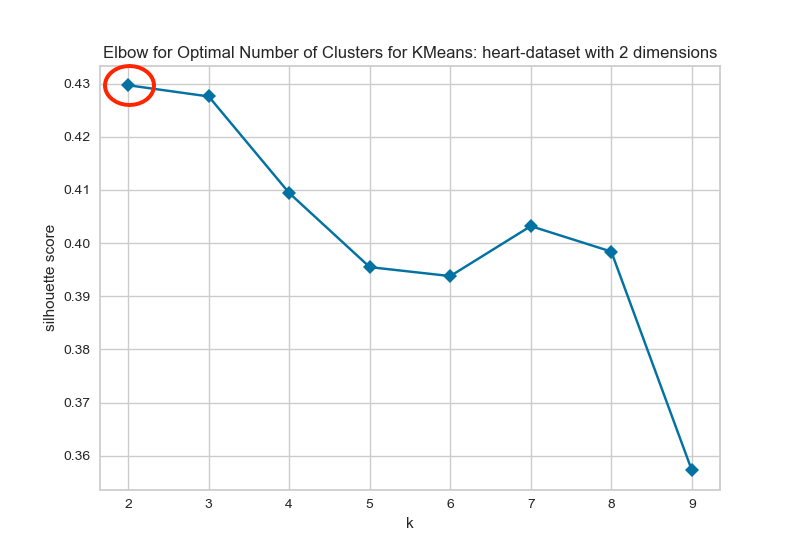
\includegraphics[width=0.75\textwidth]{Method/images/k-values/heart-dataset-2-kmeans.png}
  \caption{Selecting the $k$ for K-Means clustering for Heart dataset (2 dimensions) using the "silhouette method"}
  \label{hyperparameters:agglomerative-heart-dataset-2d}
\end{figure}
\begin{figure}[H]
  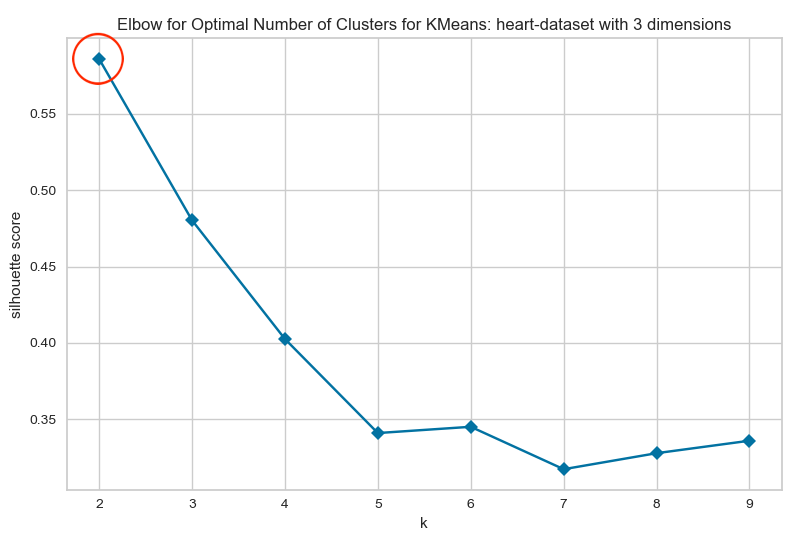
\includegraphics[width=0.75\textwidth]{Method/images/k-values/heart-dataset-3-kmeans.png}
  \caption{Selecting the $k$ for K-Means clustering for Heart dataset (3 dimensions) using the "silhouette method"}
  \label{hyperparameters:agglomerative-heart-dataset-3d}
\end{figure}
\begin{figure}[H]
  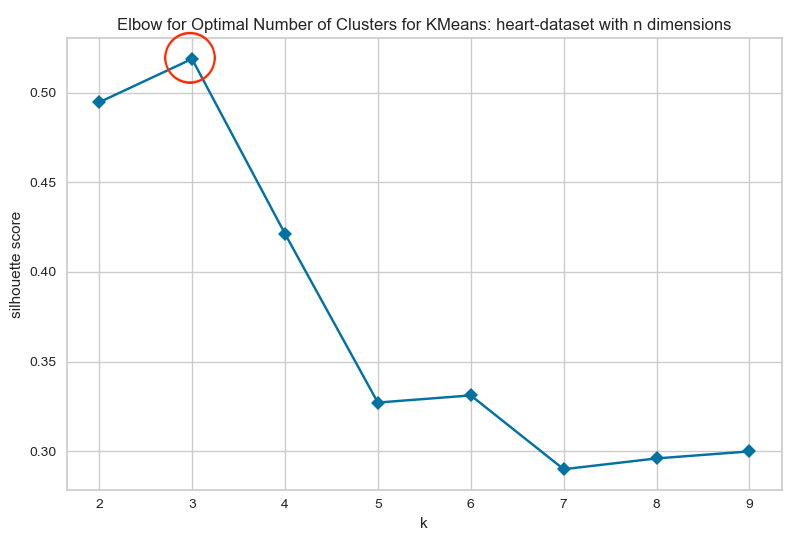
\includegraphics[width=0.75\textwidth]{Method/images/k-values/heart-dataset-n-kmeans.png}
  \caption{Selecting the $k$ for K-Means clustering for Heart dataset (9 dimensions) using the "silhouette method"}
  \label{hyperparameters:agglomerative-heart-dataset-9d}
\end{figure}
\newpage

\subsection{Circle dataset}

\begin{figure}[H]
  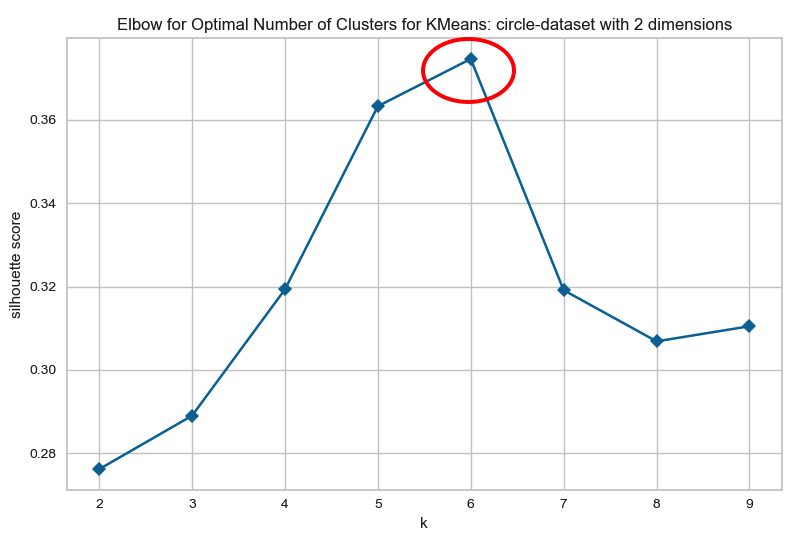
\includegraphics[width=0.75\textwidth]{Method/images/k-values/circle-dataset-2-kmeans.png}
  \caption{Selecting the $k$ for K-Means clustering for circle dataset (2-dimensions) using the "silhouette method"}
  \label{hyperparameters:agglomerative-circle-dataset-2d}
\end{figure}
\begin{figure}[H]
  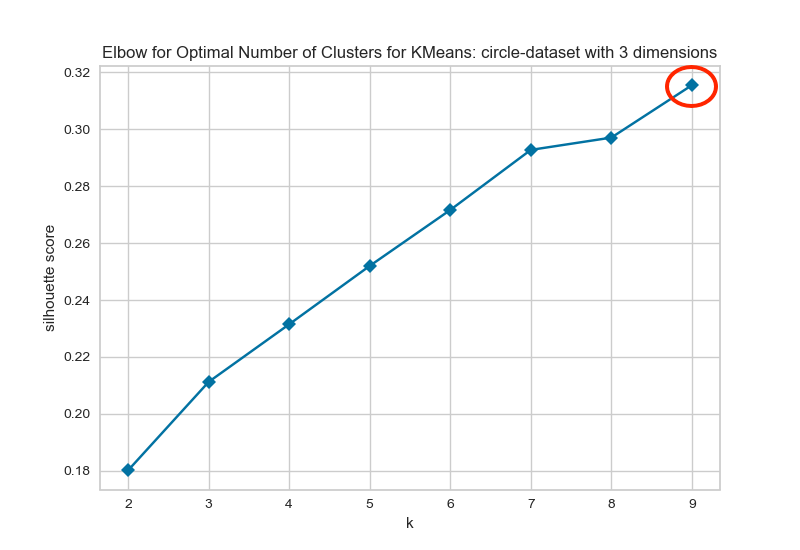
\includegraphics[width=0.75\textwidth]{Method/images/k-values/circle-dataset-3-kmeans.png}
  \caption{Selecting the $k$ for K-Means clustering for circle dataset (3-dimensions) using the "silhouette method"}
  \label{hyperparameters:agglomerative-circle-dataset-3d}
\end{figure}
\newpage

\subsection{Line dataset}
\begin{figure}[H]
  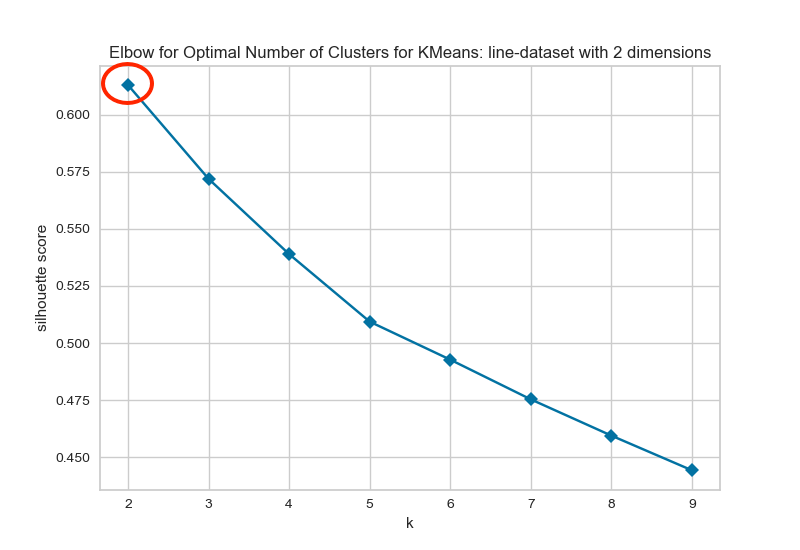
\includegraphics[width=0.75\textwidth]{Method/images/k-values/line-dataset-2-kmeans.png}
  \caption{Selecting the $k$ for K-Means clustering for line dataset (2-dimensions) using the "silhouette method"}
  \label{hyperparameters:agglomerative-line-dataset-2d}
\end{figure}
\begin{figure}[H]
  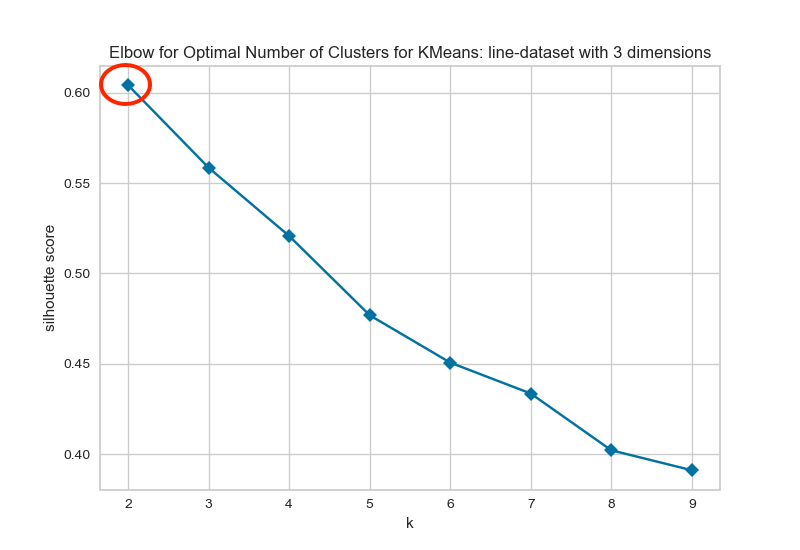
\includegraphics[width=0.75\textwidth]{Method/images/k-values/line-dataset-3-kmeans.png}
  \caption{Selecting the $k$ for K-Means clustering for line dataset (3-dimensions) using the "silhouette method"}
  \label{hyperparameters:agglomerative-line-dataset-3d}
\end{figure}
\newpage
\subsection{Skewed dataset}
\begin{figure}[H]
  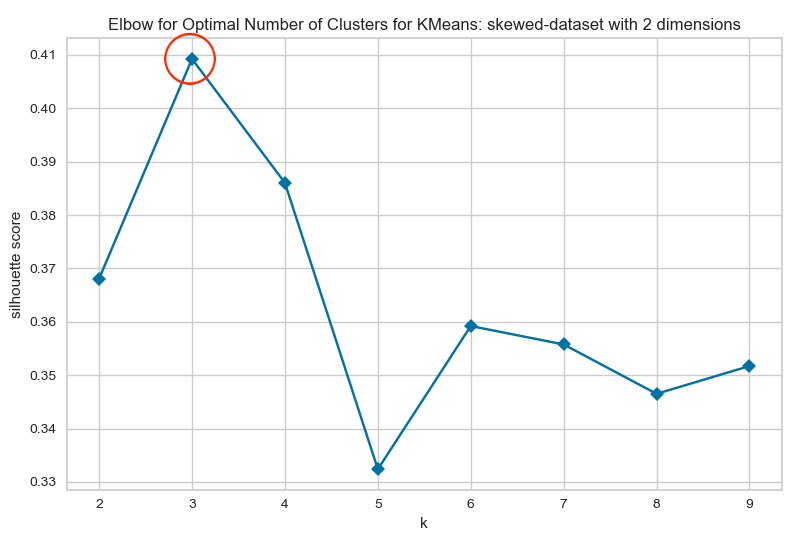
\includegraphics[width=0.75\textwidth]{Method/images/k-values/skewed-dataset-2-kmeans.png}
  \caption{Selecting the $k$ for K-Means clustering for skewed dataset (2-dimensions) using the "silhouette method"}
  \label{hyperparameters:agglomerative-skewed-dataset-2d}
\end{figure}
\begin{figure}[H]
  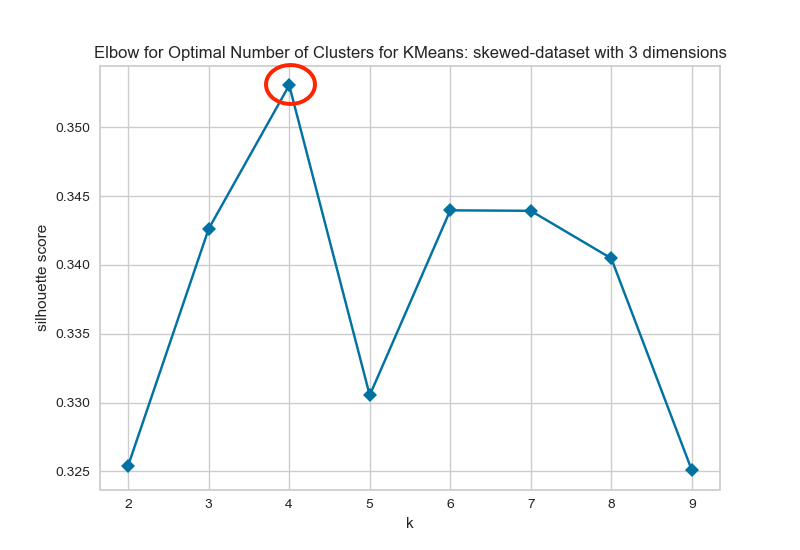
\includegraphics[width=0.75\textwidth]{Method/images/k-values/skewed-dataset-3-kmeans.png}
  \caption{Selecting the $k$ for K-Means clustering for skewed dataset (3-dimensions) using the "silhouette method"}
  \label{hyperparameters:agglomerative-skewed-dataset-3d}
\end{figure}
\newpage
\section{Agglomerative clustering} \label{appendix:agglomerative-hyperparameters}
The same as with K-Means applies to \gls{ag}.
\begin{enumerate}
    \item Seeds dataset:
    \begin{enumerate}
        \item 2-dimensions k-value: 2
        \item 3-dimensions k-value: 2
        \item 7-dimensions k-value 4
    \end{enumerate}
    \item     Heart dataset:
    \begin{enumerate}
        \item 2-dimensions k-value: 2
        \item 3-dimensions k-value: 4
        \item 9-dimensions k-value 3
    \end{enumerate}
    \item Circle dataset:
    \begin{enumerate}
        \item 2-dimensions k-value: 7
        \item 3-dimensions k-value: 9
    \end{enumerate}
    \item Line dataset (all dimensions) k-value: 
    \begin{enumerate}
        \item 2-dimensions k-value: 2
        \item 3-dimensions k-value: 3
    \end{enumerate}
    \item Skewed dataset:
    \begin{enumerate}
        \item 2-dimensions k-value: 6
        \item 3-dimensions k-value: 9
    \end{enumerate}
\end{enumerate}
\newpage
\subsection{Seeds dataset}
\begin{figure}[H]
  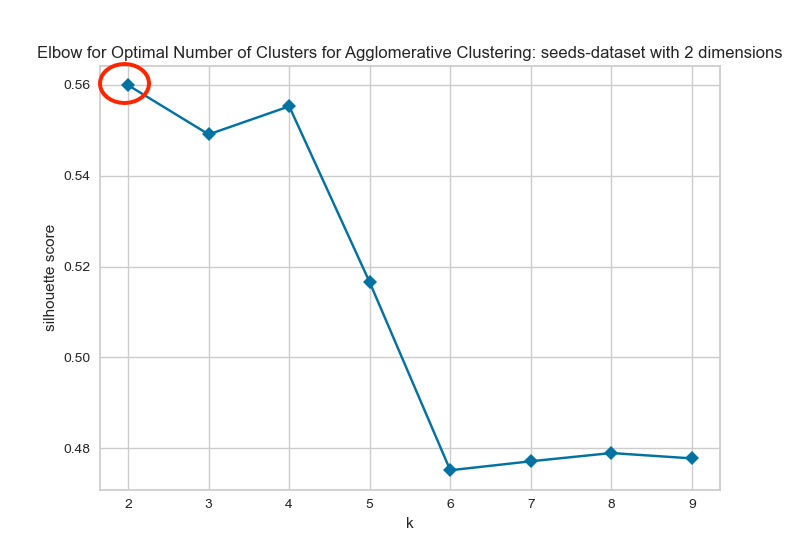
\includegraphics[width=0.75\textwidth]{Method/images/k-values/seeds-dataset-2-agglomerative.png}
  \caption{Selecting the $k$ for Agglomerative clustering for seeds dataset (2 dimensions) using the"silhouette method"}
  \label{hyperparameters:agglomerative-seeds-dataset-2d}
\end{figure}
\begin{figure}[H]
  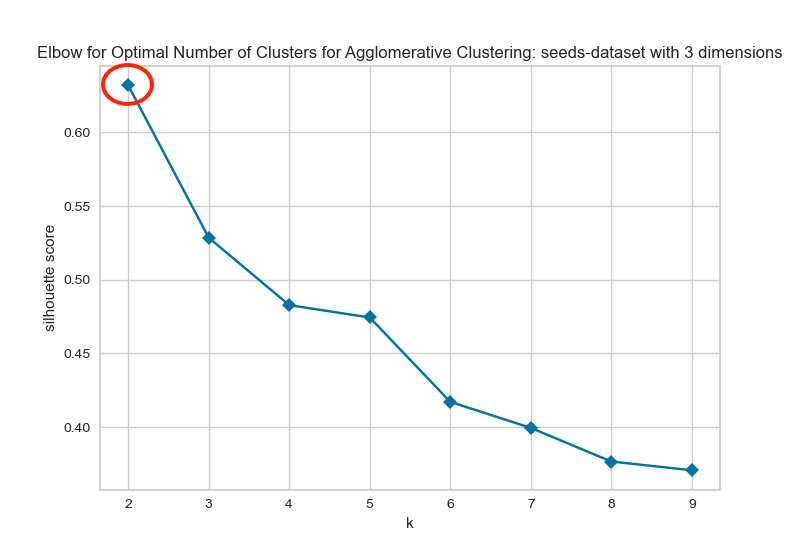
\includegraphics[width=0.75\textwidth]{Method/images/k-values/seeds-dataset-3-agglomerative.png}
  \caption{Selecting the $k$ for Agglomerative clustering for seeds dataset (3 dimensions) using the "silhouette method"}
  \label{hyperparameters:agglomerative-seeds-dataset-3d}
\end{figure}
\begin{figure}[H]
  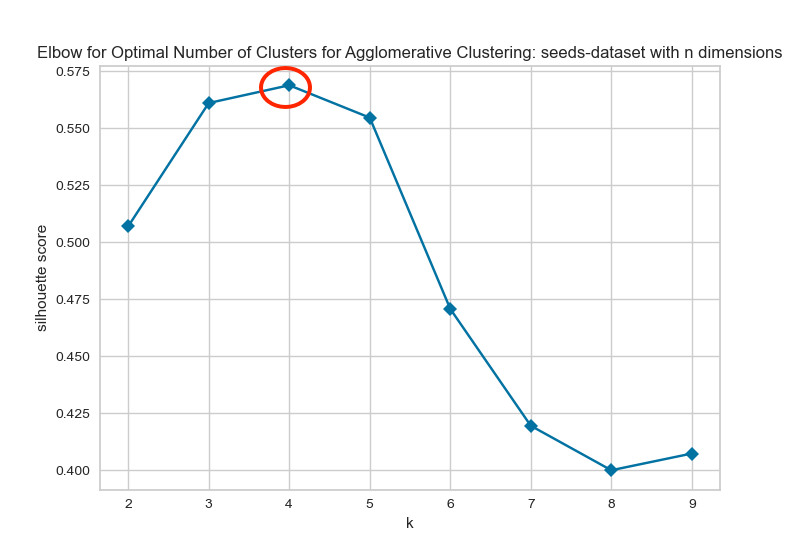
\includegraphics[width=0.75\textwidth]{Method/images/k-values/seeds-dataset-n-agglomerative.png}
  \caption{Selecting the $k$ for Agglomerative clustering for seeds dataset (7 dimensions) using the "silhouette method"}
  \label{hyperparameters:agglomerative-seeds-dataset-7d}
\end{figure}
\newpage

\subsection{Heart dataset}
\begin{figure}[H]
  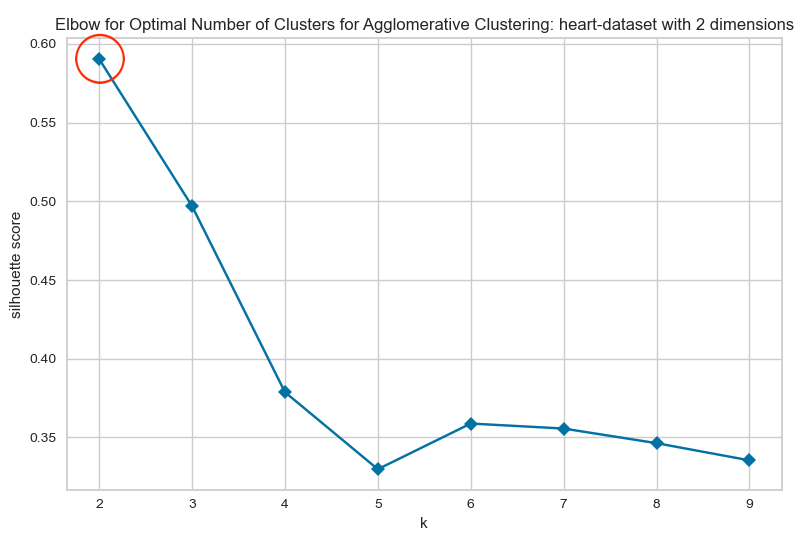
\includegraphics[width=0.75\textwidth]{Method/images/k-values/heart-dataset-2-agglomerative.png}
  \caption{Selecting the $k$ for Agglomerative clustering for Heart dataset (2 dimensions) using the "silhouette method"}
  \label{hyperparameters:agglomerative-heart-dataset-2d}
\end{figure}
\begin{figure}[H]
  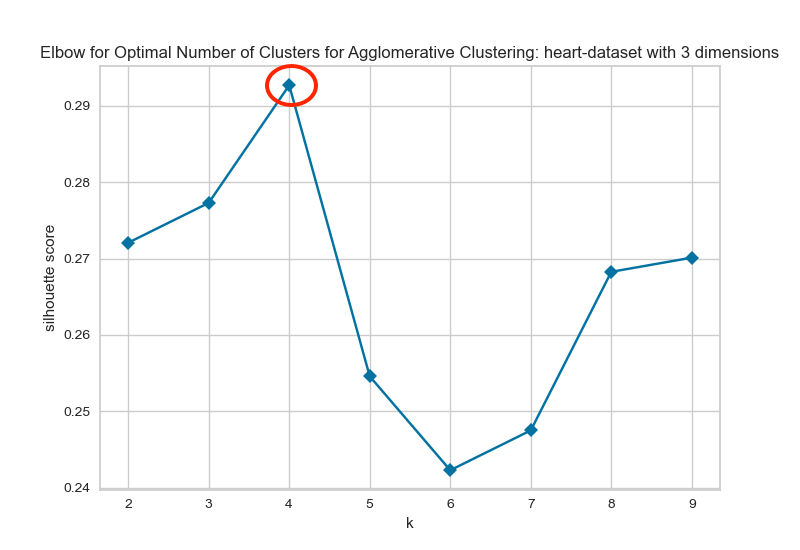
\includegraphics[width=0.75\textwidth]{Method/images/k-values/heart-dataset-3-agglomerative.png}
  \caption{Selecting the $k$ for Agglomerative clustering for Heart dataset (3 dimensions) using the "silhouette method"}
  \label{hyperparameters:agglomerative-heart-dataset-3d}
\end{figure}
\begin{figure}[H]
  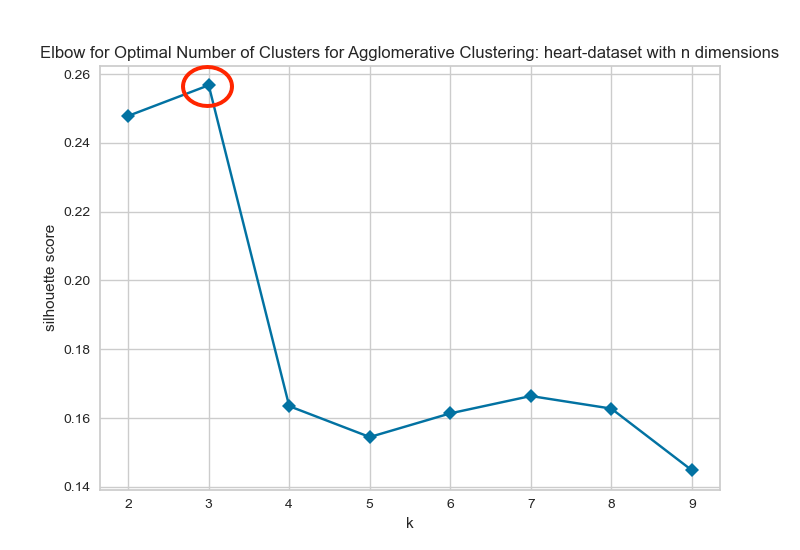
\includegraphics[width=0.75\textwidth]{Method/images/k-values/heart-dataset-n-agglomerative.png}
  \caption{Selecting the $k$ for Agglomerative clustering for Heart dataset (9 dimensions) using the "silhouette method"}
  \label{hyperparameters:agglomerative-heart-dataset-9d}
\end{figure}
\newpage

\subsection{Circle dataset}

\begin{figure}[H]
  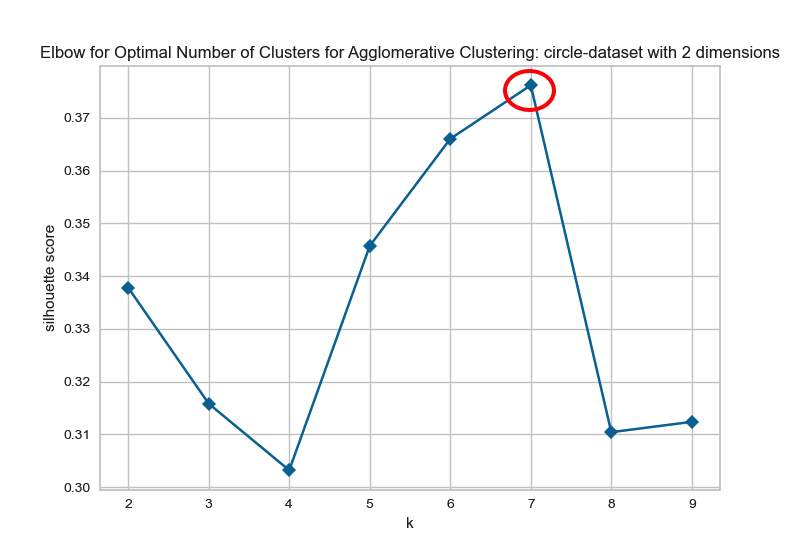
\includegraphics[width=0.75\textwidth]{Method/images/k-values/circle-dataset-2-agglomerative.png}
  \caption{Selecting the $k$ for Agglomerative clustering for circle dataset (2-dimensions) using the "silhouette method"}
  \label{hyperparameters:agglomerative-circle-dataset-2d}
\end{figure}
\begin{figure}[H]
  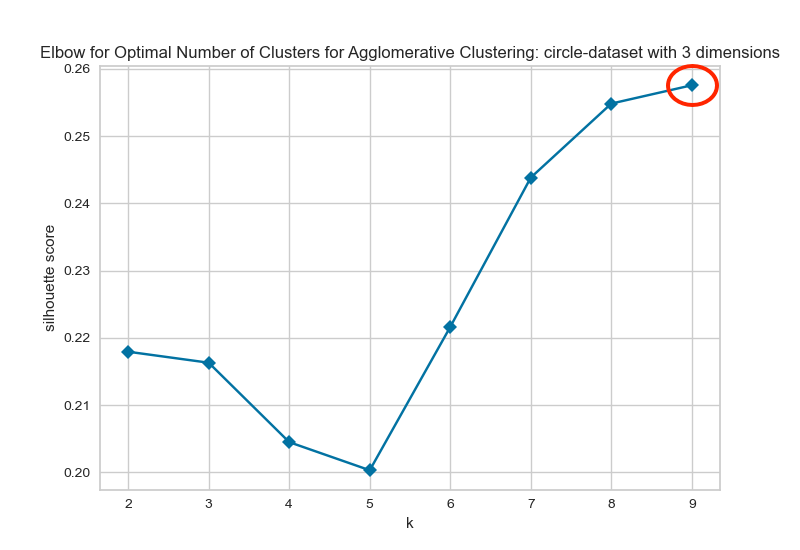
\includegraphics[width=0.75\textwidth]{Method/images/k-values/circle-dataset-3-agglomerative.png}
  \caption{Selecting the $k$ for Agglomerative clustering for circle dataset (3-dimensions) using the "silhouette method"}
  \label{hyperparameters:agglomerative-circle-dataset-3d}
\end{figure}
\newpage

\subsection{Line dataset}
\begin{figure}[H]
  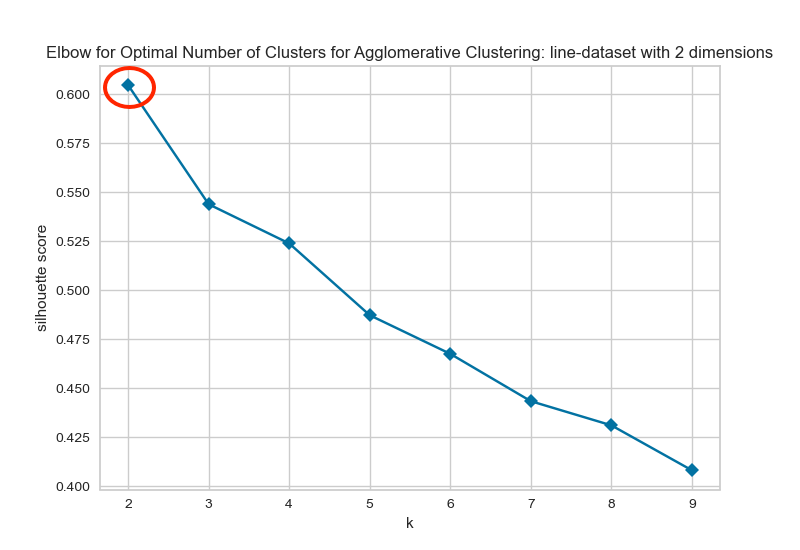
\includegraphics[width=0.8\textwidth]{Method/images/k-values/line-dataset-2-agglomerative.png}
  \caption{Selecting the $k$ for Agglomerative clustering for line dataset (2-dimensions) using the "silhouette method"}
  \label{hyperparameters:agglomerative-line-dataset-2d}
\end{figure}
\begin{figure}[H]
  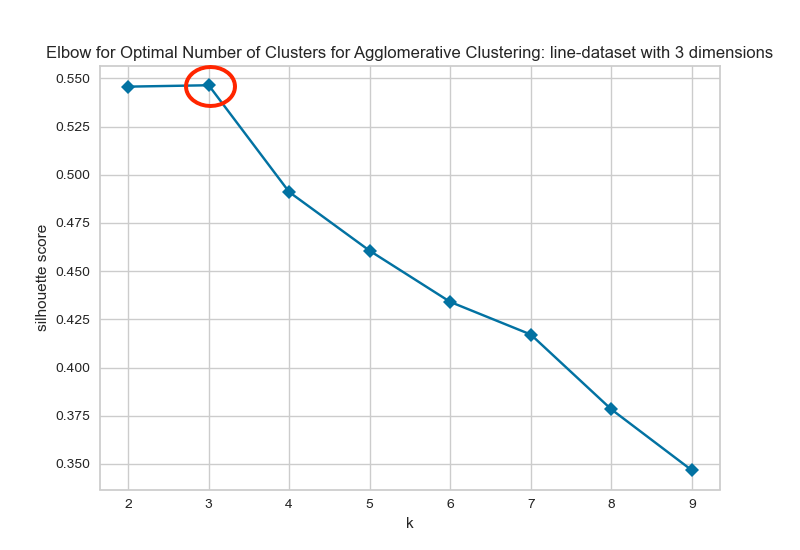
\includegraphics[width=0.75\textwidth]{Method/images/k-values/line-dataset-3-agglomerative.png}
  \caption{Selecting the $k$ for Agglomerative clustering for line dataset (3-dimensions) using the "silhouette method"}
  \label{hyperparameters:agglomerative-line-dataset-3d}
\end{figure}
\newpage
\subsection{Skewed dataset}
\begin{figure}[H]
  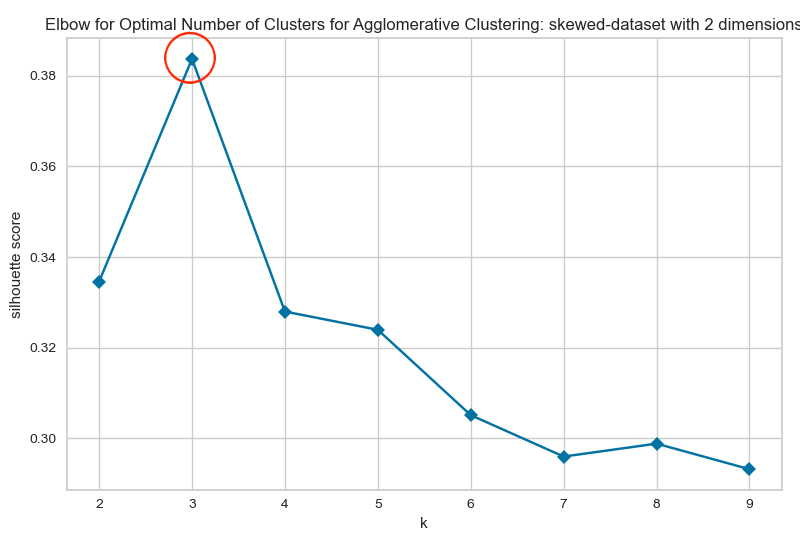
\includegraphics[width=0.75\textwidth]{Method/images/k-values/skewed-dataset-2-agglomerative.png}
  \caption{Selecting the $k$ for Agglomerative clustering for skewed dataset (2-dimensions) using the "silhouette method"}
  \label{hyperparameters:agglomerative-skewed-dataset-2d}
\end{figure}
\begin{figure}[H]
  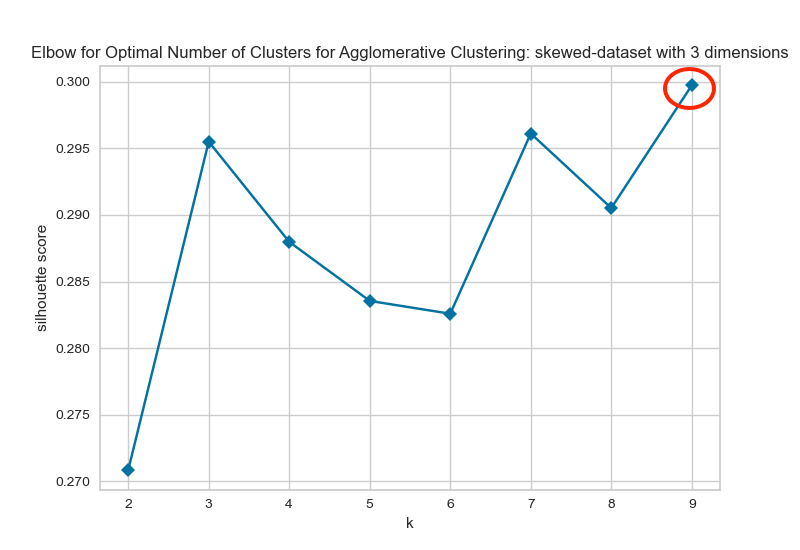
\includegraphics[width=0.75\textwidth]{Method/images/k-values/skewed-dataset-3-agglomerative.png}
  \caption{Selecting the $k$ for Agglomerative clustering for skewed dataset (3-dimensions) using the "silhouette method"}
  \label{hyperparameters:agglomerative-skewed-dataset-3d}
\end{figure}